\documentclass[10pt,aspectratio=43,mathserif]{beamer} 
\usepackage{float}
\usepackage{graphicx}
\usepackage{mathrsfs} % for mathscr
\usepackage{animate}
\usepackage{amsmath,bm,amsfonts,amssymb,enumerate,epsfig,bbm,calc,color,ifthen,capt-of,multimedia,hyperref}
\usepackage{tikz}
\usepackage{hyperref}
\usetheme{Berlin} 



\usepackage{xcolor}
\usepackage{listings}

\graphicspath{{img/}}

\definecolor{mygreen}{rgb}{0,0.6,0}
\definecolor{mygray}{rgb}{0.5,0.5,0.5}
\definecolor{mymauve}{rgb}{0.58,0,0.82}
\newcommand{\Console}{Console}
\lstset{ %
	backgroundcolor=\color{white},   % choose the background color
	basicstyle=\footnotesize\rmfamily,     % size of fonts used for the code
	columns=fullflexible,
	breaklines=true,                 % automatic line breaking only at whitespace
	captionpos=b,                    % sets the caption-position to bottom
	tabsize=4,
	commentstyle=\color{mygreen},    % comment style
	escapeinside={\%*}{*)},          % if you want to add LaTeX within your code
	keywordstyle=\color{blue},       % keyword style
	stringstyle=\color{mymauve}\ttfamily,     % string literal style
	numbers=left, 
%	frame=single,
	rulesepcolor=\color{red!20!green!20!blue!20},
	% identifierstyle=\color{red},
	language=c
}

\title{incGM+ algorithm}
\subtitle{\fontsize{9pt}{14pt}\textbf{Understanding and Implementation}}
\author{Shitong CHAI}
\institute{ISIMA}
\date{\today}

\AtBeginSection[]
{
	\begin{frame}<beamer>
	\frametitle{\textbf{table of contents}}
	\tableofcontents[currentsection]
    \end{frame}
}
\beamerdefaultoverlayspecification{<+->}
\begin{document}
\frame{\titlepage}
%\section{Table of contents}
%\begin{frame}{table of contents}
%\tableofcontents
%\end{frame}

\section{Theory}
\begin{frame}{Isomorphism and Monomorphism}

    The base graph $G$ with 4 nodes:
    \begin{equation}
    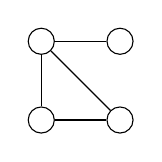
\begin{tikzpicture}
        \node[shape=circle,draw=black] (A) at (0,0) {};
        \node[shape=circle,draw=black] (B) at (0,1) {};
        \node[shape=circle,draw=black] (C) at (1,0) {};
        \node[shape=circle,draw=black] (D) at (1,1) {};
        \path [-] (A) edge node {} (B);
        \path [-] (B) edge node {} (C);
        \path [-] (A) edge node {} (C);
        \path [-] (B) edge node {} (D); 
    \end{tikzpicture}
\tag{$G$}
    \end{equation}

    has a subgraph monomorphism with path graph $S$ with 3 nodes:
    \begin{equation}
    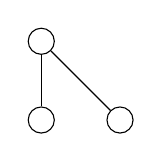
\begin{tikzpicture}
        \node[shape=circle,draw=black] (A) at (0,0) {};
        \node[shape=circle,draw=black] (B) at (0,1) {};
        \node[shape=circle,draw=black] (C) at (1,0) {};
        \path [-] (A) edge node {} (B);
        \path [-] (B) edge node {} (C); 
    \end{tikzpicture}
\tag{$S$}
    \end{equation}
    with an embedding of the same shape, but it has no subgraph isomorphisms with path graph with 3 nodes because $S$ is not an induced subgraph of $G$ with 3 nodes. Monomorphism is much slower because of larger search space and I misunderstood the paper and implemented this in the beginning XD.

\end{frame}

\begin{frame}{MNI metric}

\begin{definition}
    (MNI metric\cite{grami}) Let $f_1,\cdots,f_m$ be the set of isomorphisms of a subgraph $S(V_S,E_S)$ in a graph $G$. Also let $F(v)=\{f_1(v),\cdots,f_m(v)\}$ be the set that contains the distinct nodes in $G$ whose functions $f_1,\cdots,f_m$ map a node $v\in V_S$. The minimum image based support(MNI) of $S$ in $G$, denoted by $MNI_G(S)$, is defined as $MNI_G(S)=\min\{t:\ t=|F(v)|\ \forall v\in V_S\}$
\end{definition}

\end{frame}

\begin{frame}{Anti-monotone property of MNI}

\begin{theorem}
    (Property of MNI\cite{grami}) For a graph $G$, we have a tree $T$  whose nodes are subgraphs of $G$, say $n_T\in G$. And the tree is constructed by extending root with $n\in V(G), n\notin V(root)$ recursively. If we have subgraphs $S_1$ and $S_2$, subgraph $S_1$ is a child of subgraph $S_2$ and $S_2$ is infrequent in MNI metric, then $S_1$ is also infrequent in MNI metric.
\end{theorem}

\end{frame}

\begin{frame}{MFS and MIFS}

    Based on the \emph{Property of MNI}, all the extended graphs of infrequent subgraphs are infrequent, so there must be at least one subgraph that is the minimal one in size in the subgraph space $\mathscr{G}$, which is called Minimal InFrequent Subgraphs(MIFS). Symmetrically, we have
Maximal Frequent Subgraphs(MFS) which is the subgraphs which is maximal in size in the subgraph space $\mathscr{G}$.
A fringe is consisted of MFS and MIFS.

\end{frame}
\section{Implementation}

\begin{frame}{Data structures}
    Every (induced) subgraph is a pair $\langle G, V\rangle$ where $G$ is the base graph which is evolving, and $V$ is the nodes of the subgraph. 
    \\
    The subgraph is computed by a view object on base graph on the fly by the command G.subgraph(V) in networkx (Python package). 
    \\
    An embedding is encoded as a dictionary mapping from the node set $V$ to the node set of $G$ which can also viewed as a mapping from $G[V]$ to $G$. 
    \\
    A FELS is a pair $\langle MNI, INV \rangle$ where MNI is the MNI table of the induced subgraph $G[V]$ and $INV$ is the inverted index mapping the node of embeddings to the set(frozenset in Python) of nodes of embeddings.
\end{frame}

\begin{frame}[fragile]{incGM+}
The main function is displayed as follows, there are hundreds of lines of codes defining the data structure and functions called, but they are independent in functionality.
\begin{lstlisting}[language=python, frame=single]
def incGM_plus(G, fringe, tau, newgraph):
    G.add_edges_from(newgraph.edges)
    newnodes = frozenset(newgraph.nodes)
    fringe.addMIFS(newnodes)
    i = 0
    while 0 <= i <len(fringe.MIFS):
        S_nodes = fringe.MIFS[i]
        embeds = SEARCHLIMITED(S_nodes, newnodes,G)
        if not embeds:
            isFreq = EVALUATE(G,tau,S_nodes)
        else:
            isFreq = fels_dict.is_frequent(S_nodes, tau, G)
        delete = UPDATEFRINGE(fringe, S_nodes, isFreq, tau, G)
        i = i + 1 - int(delete)
    return fringe.MFS
\end{lstlisting}

\end{frame}
\section{result}
\begin{frame}{Example}

    \begin{figure}[H]
\centering
\includegraphics[width=0.7\textwidth]{base}
\caption{Base graph $G$}
\end{figure}

\end{frame}

\begin{frame}{Result}

    \begin{figure}[H]
\centering
\includegraphics[width=1\textwidth]{MFS1}
\caption{MFS of $G$ with minimum support $\tau=7$}
\end{figure}

\end{frame}

\begin{frame}{Result}

    \begin{figure}[H]
\centering
\includegraphics[width=1\textwidth]{MFS2}
        \caption{MFS of $G$ with minimum support $\tau=7(Cont.)$}
\end{figure}

\end{frame}

\begin{frame}{Result}

    \begin{figure}[H]
\centering
\includegraphics[width=1\textwidth]{MFS3}
        \caption{MFS of $G$ with minimum support $\tau=7(Cont.)$}
\end{figure}

\end{frame}

\begin{frame}{Time cost}
    \begin{figure}[H]
\includegraphics[width=0.7\textwidth]{time_cost}
        \caption{Time cost of adding an edge with respect to graph size}
\end{figure}

\end{frame}

\bibliography{report_bib}{}
\bibliographystyle{plain}
\end{document}
